\documentclass[twoside]{article}
\usepackage[a4paper]{geometry}
\geometry{verbose,tmargin=2.5cm,bmargin=2cm,lmargin=2cm,rmargin=2cm}
\usepackage{fancyhdr}
\pagestyle{fancy}

% nastavení pisma a češtiny
\usepackage{lmodern}
\usepackage[T1]{fontenc}
\usepackage[utf8]{inputenc}
\usepackage[czech]{babel}

% odkazy
\usepackage{url}

\usepackage{float}
% vícesloupcové tabulky
\usepackage{multirow}
\usepackage{amssymb}
\usepackage{bbold}
\usepackage{amsmath}
\usepackage{mathtools}
\usepackage{commath}

% vnořené popisky obrázků
\usepackage{subcaption}

% automatická konverze EPS 
\usepackage{graphicx} 
\usepackage{epstopdf}
\epstopdfsetup{update}

\graphicspath{{./images}}

% odkazy a záložky
\usepackage[unicode=true, bookmarks=true,bookmarksnumbered=true,
bookmarksopen=false, breaklinks=false,pdfborder={0 0 0},
pdfpagemode=UseNone,backref=false,colorlinks=true] {hyperref}

% Poznámky při překladu
\usepackage{xkeyval}	% Inline todonotes
\usepackage[textsize = footnotesize]{todonotes}
\presetkeys{todonotes}{inline}{}

%https://tex.stackexchange.com/questions/2783/bold-calligraphic-typeface
\DeclareMathAlphabet\mathbfcal{OMS}{cmsy}{b}{n}

% Zacni sekci slovem ukol
\renewcommand{\thesection}{Úkol \arabic{section}}
% enumerate zacina s pismenem
\renewcommand{\theenumi}{\alph{enumi}}

% smaz aktualni page layout
\fancyhf{}
% zahlavi
\usepackage{titling}
\fancyhf[HC]{\thetitle}
\fancyhf[HLE,HRO]{\theauthor}
\fancyhf[HRE,HLO]{\today}
 %zapati
\fancyhf[FLE,FRO]{\thepage}

% údaje o autorovi
\title{Automatické řízení: DÚ 2 - Řiditelnost}
\author{Vojtěch Michal}
\date{\today}

\begin{document}

\maketitle

% ---------------------------------
% ---------------------------------
% název sekce je generován automaticky jako: Úkol X

\newcommand{\rad}{{rad}}
\renewcommand{\norm}{{norm}}
\renewcommand{\tan}{{tan}}

\textbf{Zadání:}
Pro zkoumání odvrácené strany měsíce by se hodilo umístit komunikační družici na dráhu zdánlivě obíhající
translunární Lagrangeův bod L2 soustavy 3 těles Země-Měsíc-satelit. Tato dráha nazývaná "Halo orbita" je
zobrazena na obrázku. Výhodou by bylo, že družice by byla neustále ve spojení jak se Zemí, tak se stanicemi
na odvrácené straně Měsíce. Uvažme příklad řízení polohy družice v okolí této oběžné dráhy.

Řecká písmena $\xi$, $\zeta$, $\eta$ označují po řadě radiální, tečný a normálový směr motorů satelitu.
Veličiny k nim příslušné budu značit zkratkami dolními indexy \textit{rad}, \textit{norm} a \textit{tan}.
Například $u_\rad$, $u_\norm$ a $u_\tan$
jsou vstupy příslušné k jednotlivým motorům v pořadí radiální, normálový a tečný.


Linearizovaný a normalizovaný model pohybu satelitu okolo translunárního Lagrangeova bodu L2 je zadán jako
\begin{equation*}
	\dot{\vec{x}} = \underbrace{\begin{bmatrix}
		0 & 0 & 0 & 1 & 0 & 0\\
		0 & 0 & 0 & 0 & 1 & 0\\
		0 & 0 & 0 & 0 & 0 & 1\\
		7.3809 & 0 & 0 & 0 & 2 & 0\\
		0 & -2.1904 & 0 & -2 & 0 & 0\\
		0 & 0 & -3.1904 & 0 & 0 & 0
	\end{bmatrix}}_{\mathbf{A}} \vec{x} +  \underbrace{\begin{bmatrix}
		0\\
		0\\
		0\\
		1\\
		0\\
		0
	\end{bmatrix}}_{\mathbf{B}_\rad} u_\rad +  \underbrace{\begin{bmatrix}
		0\\
		0\\
		0\\
		0\\
		1\\
		0
	\end{bmatrix}}_{\mathbf{B}_\norm} u_\norm + \underbrace{
\begin{bmatrix}
		0\\
		0\\
		0\\
		0\\
		0\\
		1
	\end{bmatrix}}_{\mathbf{B}_\tan} u_\tan,
\end{equation*}
kde stavový vektor tvoří polohy a rychlosti a vstupy $\vec{u} = \begin{bmatrix}
	u_\rad & u_\norm & u_\tan
\end{bmatrix}$ jsou zrychlení vyvolaná tryskovými motory
ve směrech v pořadí uvedném výše.

\section{Stabilita systému}
\label{sec:ukol1}
Je tento lineární systém stabilní? Pokud ano, pak je i translunární ekvilibrium stabilní polohou. \\
\textbf{Řešení:}
Stabilitu vyšetřím pomocí vlastních čísel matice systému. Jsou to čísla
\begin{equation*}
	eig(\mathbf{A}) =
	\begin{cases}
		\pm 2.1587 & \\
		0 \pm 1.7862i & \\
		0 \pm 1.8626i \ &
	\end{cases}.
\end{equation*}
\begin{figure}
	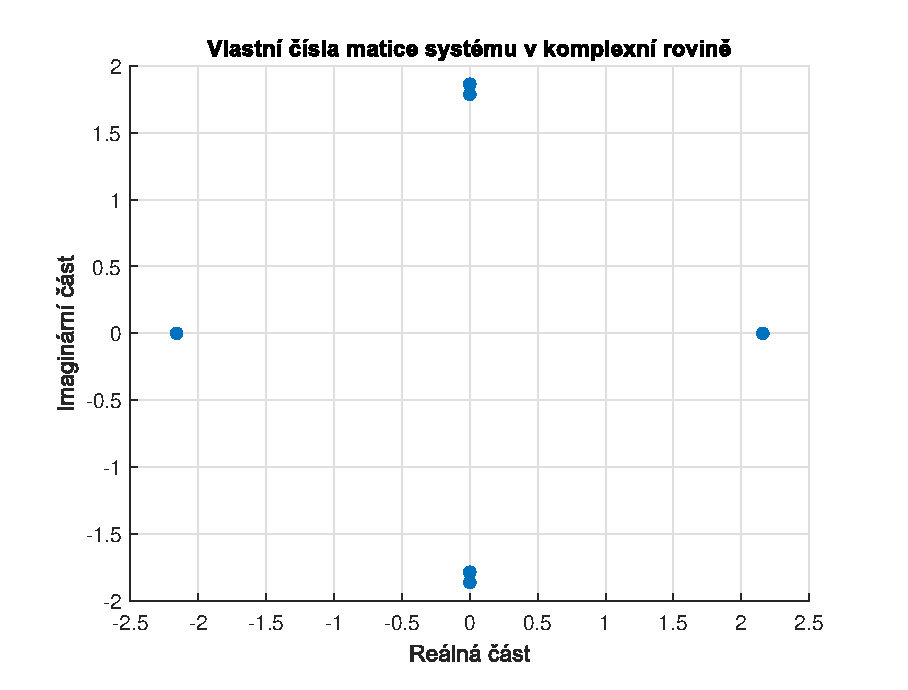
\includegraphics{vlastni_cisla.eps}
	\caption{Vlastní čísla matice $\mathbf{A}$}
	\label{fig:vlastni_cisla}
\end{figure}
Protože $\Re(2.1587) > 0$, je alespoň jedno vlastní číslo v pravé polorovině s a systém stabilní není.
To je očekávatelné, jinak by družice nepotřebovala motory žádné. 

\section{Řiditelnost jedním vstupem}
\label{sec:ukol2}
Pokud není, zjistěte kterým vstupem (a tedy kterým tryskovým motorem) je systém řiditelný. \\
\textbf{Řešení:}
Pro analýzu řiditelnosti sestrojím matice řiditelnosti z definice
\begin{equation}
	\mathbfcal{C}_\rad = \begin{bmatrix}
		\mathbf{B}_\rad & \mathbf{A}\mathbf{B}_\rad & \mathbf{A}^2 \mathbf{B}_\rad & \cdots \mathbf{A}^5 \mathbf{B}_\rad
	\end{bmatrix},
	\label{eq:riditelnost}
\end{equation}
analogicky pro směry normálový a tečný.\\
Postačující podmínka pro úplnou řiditelnost systému je, že hodnost matice řiditelnosti $\mathbfcal{C}$ je rovna řádu systému $n=6$. Protože platí
\begin{equation*}
	\begin{split}
		\text{rank}(\mathbfcal{C}_\rad) &= 4, \\
		\text{rank}(\mathbfcal{C}_\norm) &= 4, \\
		\text{rank}(\mathbfcal{C}_\tan) &= 2, \\
	\end{split}
\end{equation*}
není žádný z motorů schopen samostatně zajistit úplnou řiditelnost systému.

\section{Přenos dílčích vstupů na stav}
\label{sec:ukol3}
Vypočtěte postupně pro každý vstup (tryskový motor) přenos na stav. Poznáte z nich totéž, co jste zjistili
v bodu 2? \\
\textbf{Řešení:}
Přenos ze vstupů na stav je dán maticí 
\begin{equation*}
	\mathbf{G}_{\text{smer}} = (s\mathbf{I}-\mathbf{A})^{-1} \mathbf{B}_{\text{smer}},
\end{equation*}
kde za \textit{smer} lze dosadit dílčí směry \textit{rad}, \textit{norm} a \textit{tan}.
Pro lepší čitelnost označím $a(s) = (s+2.1587)(s^2+3.4694)(s-2.1587)$. Přenosy dílčích vstupů na stavy jsou
\begin{equation}
	\label{eq:prenosy}
	\mathbf{G}_\rad(s) = \begin{bmatrix}
		
		\frac{1.0000(s^2+2.1904)     }{a(s)}          \\                
		\frac{-2.0000s        }{a(s)}                   \\               
		0                                    \\            
		\frac{1.0000s(s^2+2.1904)}{a(s)}              \\
		\frac{-2.0000s^2}{a(s)}                         \\               
		0                                                
	\end{bmatrix}, ~~~~~~~~~                                                    
		\mathbf{G}_\norm(s) =                       
		\begin{bmatrix}
			
			\frac{2.0000s}{a(s)}                                               \\
			\frac{1.0000(s+2.7168)(s-2.7168) }{a(s)}                \\           
			0                                        \\             
			\frac{2.0000s^2                  }{a(s)}           \\
			\frac{1.0000s(s+2.7168)(s-2.7168)}{a(s)}             \\              
			0                                                     
		\end{bmatrix}, ~~~~~~~~~
		\mathbf{G}_\tan(s) = \begin{bmatrix}
			
			0                              \\   
			0                             \\    
			\frac{1.0000}{s^2+3.1904}     \\       
			0                              \\
			0                               \\   
			\frac{1.0000s}{s^2+3.1904}                           
		\end{bmatrix}.
\end{equation}
Každý z přenosů $\mathbf{G}_\rad(s)$, $\mathbf{G}_\norm(s)$, $\mathbf{G}_\tan(s)$ obsahuje nulové řádky a není proto schopen ovlivnit 
úplně všechny stavy, jak plyne již z \ref{sec:ukol2}. Pro splnění nutné podmínky úplné řiditelnosti musí být v 
každém řádku matice přenosů alespoň jeden nenulový prvek. Toho se v našem případě dá dosáhnout
například použitím motorů ve směru tečném a radiálním. Naopak motory radiální a normálový jsou ve smyslu ovlivnění
stavového prostoru lineárně závislé a použití obou dvou nijak nezvětší množinu dosažitelných stavů.

\section{Řiditelnost všemi vstupy}
\label{sec:ukol4}
Uvažte nyní celý systém se třemi vstupy a ověřte jeho řiditelnost. \\
\textbf{Řešení:}
O řiditelnosti lze rozhodnout podle kritérií uvedených v \ref{sec:ukol2}.
Pro výpočet  matice řiditelnosti pro celý systém si pomohu funkcí $ctrb$ vestavěnou do Matlabu. Protože
\begin{equation*}
	\text{rank}(\text{ctrb}(\mathbf{A}, \mathbf{B})) = 6 = n,
\end{equation*}
je systém se všemi třemi motory úplně řiditelný.

\section{Přenosová matice všech vstupů na stav}
\label{sec:ukol5}
Vypočtete přenosovou matici ze vstupů na stav pro celý systém.\\
\textbf{Řešení:}
Stejně jako v případě \ref{sec:ukol3} určím přenos $\mathbf{G}_{\text{stav}}$ ze vstupů na stav pomocí vztahu \eqref{eq:prenosy}.
Tentokrát se však použije celá matice $\mathbf{B}$ rozměrů 6x3. Stejný výsledek dá spojení vektorů $\begin{bmatrix}
	\mathbf{G}_\rad & \mathbf{G}_\norm & \mathbf{G}_\tan)
\end{bmatrix}$ z rovnice \eqref{eq:prenosy}
\begin{equation*}
	\mathbf{G}_\text{stav} = \begin{bmatrix}
	\frac{1.0000(s^2+2.1904)     }{a(s)} 	&\frac{2.0000s}{a(s)}                     & 0                             \\
	\frac{-2.0000s        }{a(s)}        	&\frac{1.0000(s+2.7168)(s-2.7168) }{a(s)} & 0                             \\
	0                                    	&0                                        & \frac{1.0000}{s^2+3.1904}     \\
	\frac{1.0000s(s^2+2.1904)}{a(s)}     	&\frac{2.0000s^2                  }{a(s)} & 0                             \\
	\frac{-2.0000s^2}{a(s)}              	&\frac{1.0000s(s+2.7168)(s-2.7168)}{a(s)} & 0                             \\
	0                                    	&0                                        & \frac{1.0000s}{s^2+3.1904}    
	\end{bmatrix}.
\end{equation*}


% ---------------------------------
% ---------------------------------
% Literatura
\begin{thebibliography}{9}


\bibitem{Wiki}
	\LaTeX tutorials, \url{http://en.wikibooks.org/wiki/LaTeX/}

\bibitem{motivace}
	Motivační hudba, \emph{Kirby dream land theme song} \url{https://www.youtube.com/watch?v=3CS93CdMv_E}

\end{thebibliography}












\end{document}

